\documentclass[fleqn]{beamer}

% This file is a solution template for:

% - Giving a talk on some subject.
% - The talk is between 15min and 45min long.
% - Style is ornate.
 


% Copyright 2004 by Till Tantau <tantau@users.sourceforge.net>.
%
% In principle, this file can be redistributed and/or modified under
% the terms of the GNU Public License, version 2.
%
% However, this file is supposed to be a template to be modified
% for your own needs. For this reason, if you use this file as a
% template and not specifically distribute it as part of a another
% package/program, I grant the extra permission to freely copy and
% modify this file as you see fit and even to delete this copyright
% notice. 


\mode<presentation>
% {
%   \usetheme{Warsaw}
%   % or ...

%   \setbeamercovered{transparent}
%   % or whatever (possibly just delete it)
% }

\usepackage{beamerthemeshadow}
\usepackage[english,czech]{babel}
\usepackage{bibentry}
%\usepackage{natbib}
%\selectbiblanguage{czech}
\usepackage{url}
\usepackage{hyperref}
\usepackage{lmodern}
\def\uv#1{\glqq#1\grqq}
\usepackage{graphicx}
%\usepackage{listings}
% or whatever
\usepackage{amsmath}
\usepackage{xspace}
\usepackage{natbib}
\usepackage{float}
%\usepackage{wrapfig}
%\usepackage{sidecap}
%\usepackage{txfonts}            
\usepackage{color}
\usepackage{verbatim}
\usepackage{listings}


\usepackage[utf8]{inputenc}
% or whatever

%\usepackage{times}
\usepackage[T1]{fontenc}
% Or whatever. Note that the encoding and the font should match. If T1
% does not look nice, try deleting the line with the fontenc.


\title[Computers in Science] % (optional, use only with long paper titles)
{Practical Astroinformatics} 

\subtitle{... or what I wish to knew when I was younger} % (optional)

\author[Jaroslav Vážný] % (optional, use only with lots of authors)
{Jaroslav Vážný / Masaryk University }
% - Use the \inst{?} command only if the authors have different
%   affiliation.

\institute[Universities of Somewhere and Elsewhere] % (optional, but mostly needed)
{

    
\includegraphics[height=2cm]{logo}

}

\date{SoftComp reg. č. CZ.1.07/2.3.00/20.0072}

% - Use the \inst command only if there are several affiliations.
% - Keep it simple, no one is interested in your street address.

%\date[Short Occasion] % (optional)
%{Date / Occasion}

\subject{Talks}
% This is only inserted into the PDF information catalog. Can be left
% out. 



% If you have a file called "university-logo-filename.xxx", where xxx
% is a graphic format that can be processed by latex or pdflatex,
% resp., then you can add a logo as follows:

\pgfdeclareimage[height=1.5cm]{logo}{logo}


%\logo{\pgfuseimage{{logo}}}


% Delete this, if you do not want the table of contents to pop up at
% the beginning of each subsection:
\AtBeginSubsection[]
{
  \begin{frame}<beamer>{Outline}
    \tableofcontents[currentsection,currentsubsection]
  \end{frame}
}


% If you wish to uncover everything in a step-wise fashion, uncomment
% the following command: 

%\beamerdefaultoverlayspecification{<+->}


\begin{document}
% vylepseny listing z http://texnik.de/TeXnik/listings/listing0.pdf
 \definecolor{hellgelb}{rgb}{1,1,0.8}
 \definecolor{colKeys}{rgb}{0,0,1}
 \definecolor{colIdentifier}{rgb}{0,0,0}
 \definecolor{colComments}{rgb}{1,0,0}
 \definecolor{colString}{rgb}{0,0.5,0}
 \lstset{%
   language={SQL},%
    morekeywords={AND,ASC,avg,CHECK,COMMIT,count,DECODE,DESC,DISTINCT,%
                 GROUP,IN,LIKE,NUMBER,ROLLBACK,SUBSTR,sum,VARCHAR2}%
 }

 \lstset{%
     float=hbp,%
     basicstyle=\ttfamily\small, %
%     identifierstyle=\color{colIdentifier}, %
%     keywordstyle=\color{colKeys}, %
     stringstyle=\color{colString}, %
     commentstyle=\color{colComments}, %
     columns=flexible, %
     tabsize=4, %
     frame=single, %
     extendedchars=true, %
     showspaces=false, %
     showstringspaces=false, %
   numbers=left, %
   numberstyle=\tiny, %
   breaklines=true, %
   backgroundcolor=\color{hellgelb}, %
   breakautoindent=true, %
   captionpos=b%
 }

 




\begin{frame}
  \titlepage
\end{frame}


%\begin{frame}
%  \tableofcontents
%\end{frame}


\begin{section}{Motivation}     
 \begin{frame}
   \begin{center}
     \frametitle{Prelude}
     \small{motto:  The only way to keep away from computers in
       science is to understand them ... }
   \end{center}

     \vspace{1cm}
    \tiny{ \url{https://www.coursera.org/}}

 \end{frame}
\end{section}


\begin{section}{Overview}
\begin{frame}\frametitle{Concepts introduced in this talk}
  \begin{center}
    \vspace{1cm}
    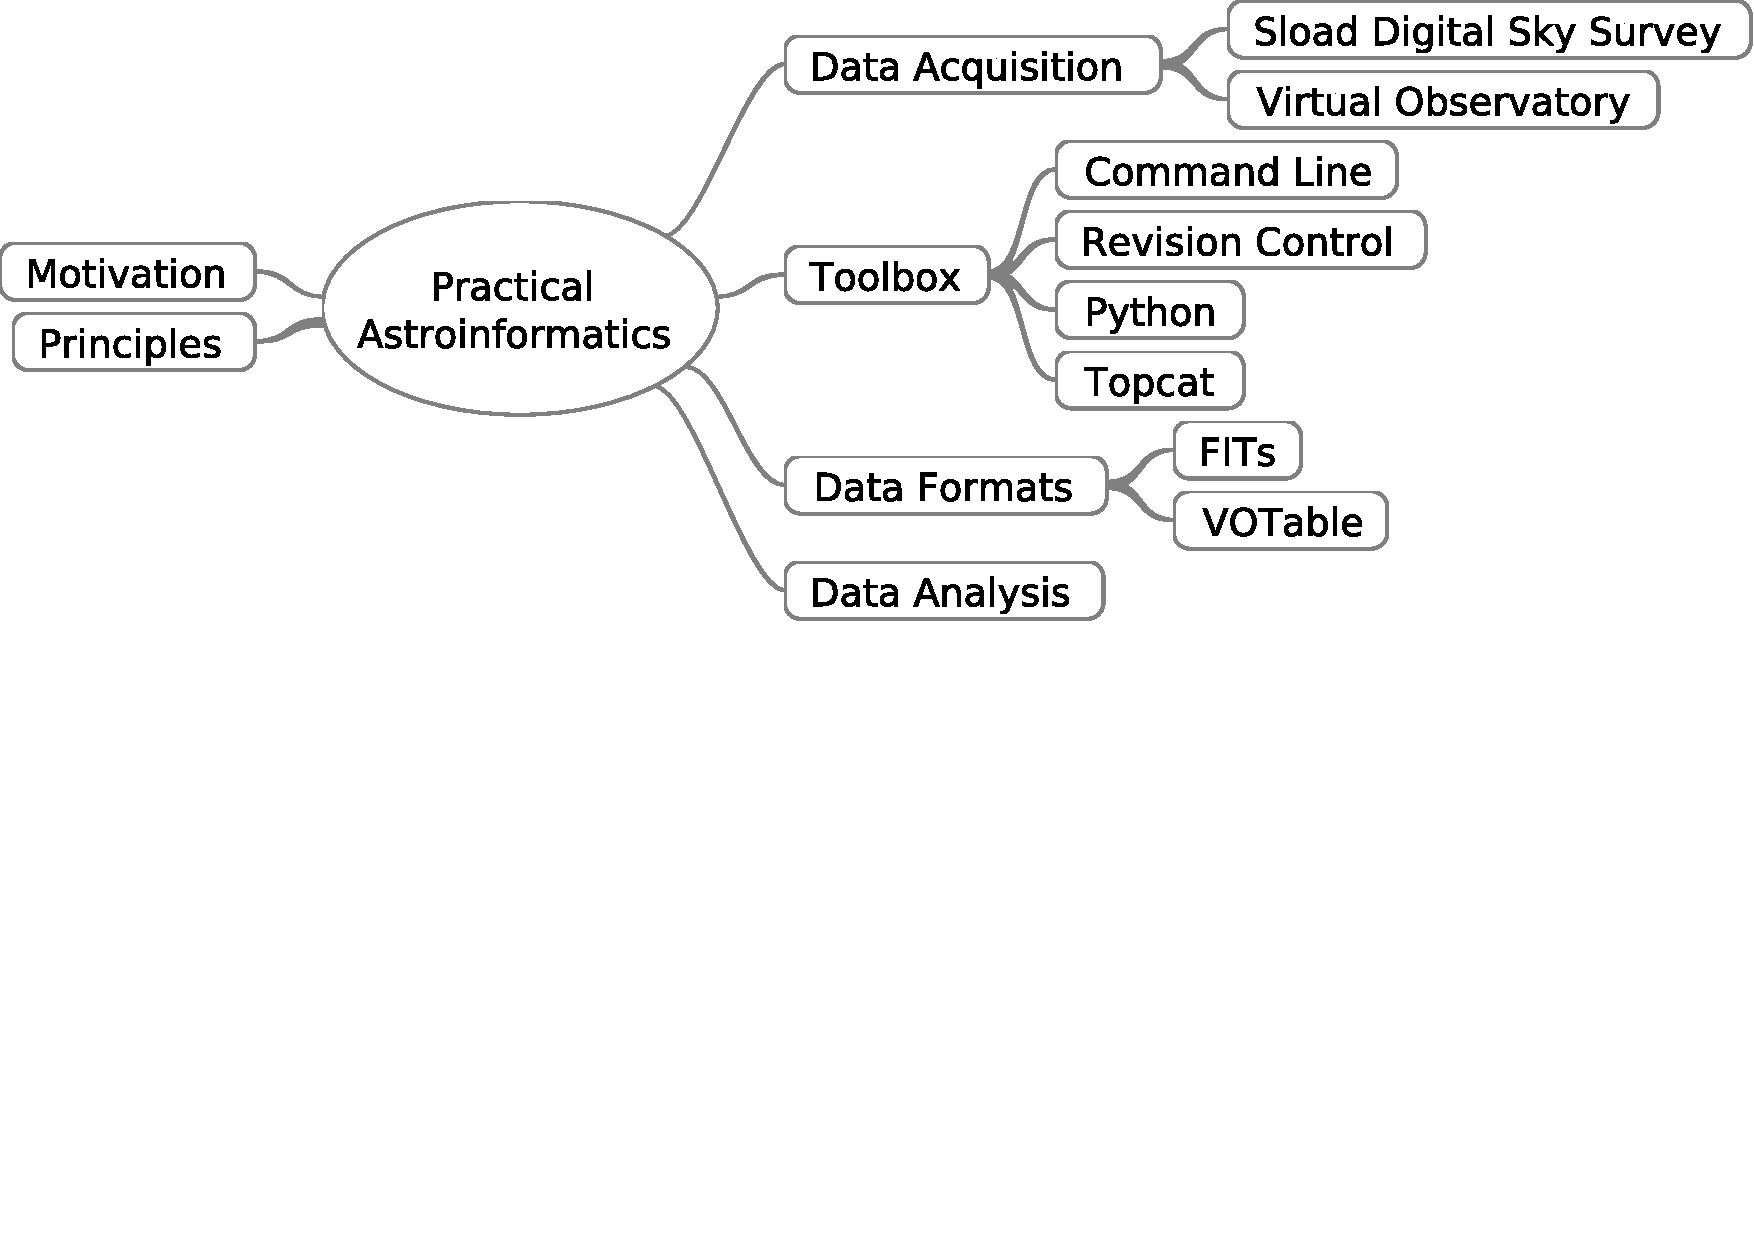
\includegraphics[width=1.0\textwidth]{overview}    
  \end{center}
\end{frame}
\end{section}

  \begin{frame}\frametitle{Data Avalanche?}
  \begin{itemize}
    \item{Large Synoptic Survey Telescope}
      \begin{itemize}
        \item 20 TB per night
        \item 60 PB for the raw data (after 10 years)
        \item 15 PB for the catalog database
        

      \end{itemize}



        \small{The total data volume after processing will be
        several hundred PB}

          \bigskip

    \item{Where I can learn more?}
      \begin{itemize}
       \item \url{http://www.lsst.org/}
      \end{itemize}
  \end{itemize}
  \end{frame}

\begin{section}{Data Acquisition}
  \begin{frame}\frametitle{Sloan Digital Sky Survey}
  \begin{itemize}
    \item{Why is it important?}
      \begin{itemize}
        \item Lots of data (>$10^6$ objects)
        \item Perfect documentation
        \item Tools to access the data
      \end{itemize}
    \item{Where I can learn it?}
      \begin{itemize}
       \item \url{http://www.sdss3.org/}
      \end{itemize}
  \end{itemize}
  \end{frame}

  \begin{frame}\frametitle{Virtual Observatory}
  \begin{itemize}
    \item{Why is it important?}
      \begin{itemize}
        \item Uniform access to astronomy data
        \item Based on Web standards
        \item Many tools with vo support (Topcat, Aladin, Tapsh)
      \end{itemize}
    \item{Where I can learn it?}
      \begin{itemize}
       \item \url{http://physics.muni.cz/~vazny/wiki/index.php/Diploma_work}
      \end{itemize}
  \end{itemize}
  \end{frame}


% Protocols
\begin{frame}[containsverbatim]\frametitle{Example: Virtual
    Observatory Protocols}

Cone Search Protocol

\begin{lstlisting}
http://simbad.u-strasbg.fr/simbad-conesearch.pl?RA=24.5&DEC=-57.2&SR=0.1
\end{lstlisting}


Simple Image Access Protocol

\begin{lstlisting}
  http://hubblesite.org/cgi-bin/sia/hst_pr_sia.pl?POS=83.6,22.0&SIZE=1.0
\end{lstlisting}

Simple Spectra Access Protocol

\begin{lstlisting}
  http://archive.eso.org/apps/ssaserver/EsoProxySsap?REQUEST=queryData&POS=83.63,22&SIZE=1
\end{lstlisting}

\end{frame}

\begin{frame}[containsverbatim]\frametitle{Example: Virtual
    Observatory Protocols}

Table Access Protocol
\begin{lstlisting}
  -- Display all identifiers of a given object.
  SELECT id2.id
  FROM ident AS id1 JOIN ident AS id2 USING(oidref)
  WHERE id1.id = 'M1';
\end{lstlisting}

\url{http://simbad.u-strasbg.fr/simbad/sim-tap}

\end{frame}

\end{section}


% ToolBox

\begin{section}{ToolBox}

  \begin{frame}\frametitle{Command Line}
  \begin{itemize}
    \item{Why is it important?}
    \begin{itemize}
      \item{Efficient dialog computer $\Longleftrightarrow$ human}
      \item{In all advanced tools (Programming, mathematica, CAD, \ldots)}
      \item{Cooperation, re-usability, automatize }
    \end{itemize}

    \item{Where I can learn it?}
    \begin{itemize}
      \item PEEPCODE: Meet the Command Line, Advanced Command Line  
    \end{itemize}
  \end{itemize}


  \end{frame}

  \begin{frame}\frametitle{Examples}
  \begin{itemize}
    \item TAB, CTRL-A, CTRL-E (=Emacs)
    \item !! Repeat last command
    \item !\$ Repeat last agrument
    \item history command history
    \item CTRL+R search in history
  \end{itemize}
  \end{frame}

  
  \begin{frame}\frametitle{Text tools}
  \begin{itemize}
    \item{Why is it important?}
      \begin{itemize}
      \item "Everything" is a text
      \item head, tail, sed, awk, join, paste, vim, emacs \ldots
      \end{itemize}
 \item{Where I can learn it?}
  \begin{itemize}
      \item PEEPCODE: Meet Emacs, Smash Into Vim, Vim Emacs tutorials
  \end{itemize}
  \end{itemize}
  \end{frame}

  \begin{frame}\frametitle{Revision Control Systems}
  \begin{itemize}
    \item{Why is it important?}
      \begin{itemize}
      \item Distributed systems (Git, Mercurial)
      \item Almost everything is local
      \item Branching
      \item Natural (subjective?)
      \end{itemize}
    \item{Where I can learn it?}
      \begin{itemize}
        \item PEEPCODE: Git, Mercurial
        \item \url{https://github.com}
        \item \url{http://gitref.org/}
        \item \url{http://www.youtube.com/watch?v=ZDR433b0HJY}

      \end{itemize}
  \end{itemize}
  \end{frame}


  \begin{frame}\frametitle{Python}
  \begin{itemize}
    \item{Why is it important?}
      \begin{itemize}
      \item Language of science ? 
      \item Cooperation between scientist (Scipy conference)
      \item Perfect for experiments (\href{http://ipython.org/ipython-doc/rel-0.12/_static/notebook_specgram.png}{iPython})
      \item Real free language (!= MATBLAB)

      \end{itemize}
    \item{Where I can learn it?}
      \begin{itemize}
      \item \url{http://pyvideo.org/}
      \item \url{http://www.youtube.com/watch?v=B9MvjMFokLc}
      \item \url{http://ipython.org/}

      \end{itemize}
  \end{itemize}
  \end{frame}


  \begin{frame}\frametitle{Topcat}
  \begin{itemize}
    \item{Why is it important?}
      \begin{itemize}
      \item Perfect for big data (not only astro) 
      \item Example of cooperation between GUI applications
      \item Learning Astrophysics

      \end{itemize}
    \item{Where I can learn it?}
      \begin{itemize}
      \item \url{http://www.star.bris.ac.uk/~mbt/topcat/}
      \item \url{http://www.eurovo-ice.eu/twiki/bin/view/EuroVOICE/ICESchool}

      \end{itemize}
  \end{itemize}
  \end{frame}



% Data formats

\begin{section}{Data Formats}
  %% \begin{frame}\frametitle{ASCII}
  %% \begin{itemize}
  %%   \item{Why is it important?}
  %%   \item{Where I can learn it?}
  %% \end{itemize}
  %% \end{frame}

  \begin{frame}\frametitle{FITs}
  \begin{itemize}
    \item{Why is it important?}
      \begin{itemize}
      \item De-Facto standard in Astronomy
      \item Flexible, Efficient, ASCII Meta-Data
      \end{itemize}
    \item{Where I can learn it?}
      \begin{itemize}
      \item \url{http://fits.gsfc.nasa.gov}
      \end{itemize}
  \end{itemize}
  \end{frame}

\begin{frame}[containsverbatim]\frametitle{Example: Reading FITS file}
\begin{lstlisting}[language=SQL]
In [1]: import pyfits
In [2]: hdulist = pyfits.open('spSpec-53237-1886-248.fit')
In [3]: hdulist.info()
Filename: spSpec-53237-1886-248.fit
No.    Name         Type      Cards   Dimensions   Format
0    PRIMARY     PrimaryHDU     213  (3874, 5)     float32
1                BinTableHDU     54  6R x 23C      [1E, 1E, ...
2                BinTableHDU     54  44R x 23C     [1E, 1E, ...
3                BinTableHDU     18  1R x 5C       [1E, 1E, ...
4                BinTableHDU     32  53R x 12C     [1J, 1J, ...
5                BinTableHDU     26  36R x 9C      [19A, 1E, ...
6                BinTableHDU     14  3874R x 3C    [1J, 1J, 1E]
\end{lstlisting}
\end{frame}



%% VOTable

  \begin{frame}\frametitle{VOTable}
  \begin{itemize}
    \item{Why is it important?}
      \begin{itemize}
      \item Standard in Virtual Observatory
      \item Flexible, Efficient, XML
      \end{itemize}
    \item{Where I can learn it?}
      \begin{itemize}
      \item \url{http://www.ivoa.org}
      \end{itemize}
  \end{itemize}
  \end{frame}

\begin{frame}[containsverbatim]\frametitle{Example: VOTable}
\begin{lstlisting}[language=SQL]
<?xml version="1.0" encoding="utf-8"?>
 xmlns:xsi="http://www.w3.org/2001/XMLSchema-instance"
 xsi:noNamespaceSchemaLocation="http://www.ivoa.net/xml/VOTable/v1.0"
 xmlns="http://www.ivoa.net/xml/VOTable/v1.0">
 <RESOURCE type="results" >
  <TABLE >
   <FIELD ID="col0" name="wave" datatype="float" unit=""
   precision="F9"/>
  <DATA>
    <TABLEDATA>
     <TR>
      <TD>4012.50757</TD>
     </TR>
 </TABLEDATA>
   </DATA>
  </TABLE>
 </RESOURCE>
</VOTABLE>
\end{lstlisting}
\end{frame}





%%   \begin{frame}\frametitle{Post-relational Databases}
%%   \begin{itemize}
%%     \item{Why is it important?}
%%     \item{Where I can learn it?}
%%   \end{itemize}

%%   \end{frame}



\begin{frame}[containsverbatim]\frametitle{Example: Working with FITs
    in Python}
\begin{lstlisting}[language=SQL]
  In [1]: import atpy
  In [2]: tbl = atpy.Table('spSpec-53401-2052-458.fit')
  Auto-detected input type: fits
  In [3]: tbl.write('votableExample.xml')
  Auto-detected input type: vo
\end{lstlisting}
Updating FITS file.

\begin{lstlisting}
  In [1]: prihdr = hdulist[0].header
  In [2]: prihdr.update('observer', 'Astar')
  In [3]: prihdr.add_history('Updated  3/27/11')
\end{lstlisting}

\end{frame}
\end{section}


  \begin{frame}\frametitle{Data Mining}
  \begin{itemize}
    \item{Why is it important?}
      \begin{itemize}
      \item Astrology of data
      \item Data preprocessing
      \end{itemize}
    \item{Where I can learn it?}
      \begin{itemize}
      \item {Standford(Andrew Ng)}
      \item {\url{www.avc.cvut.cz}}
      \end{itemize}
  \end{itemize}
  \end{frame}

\begin{frame}[containsverbatim]\frametitle{Example: Decison Tree}

\begin{lstlisting}
ug <= 0.663668
|   gr <= -0.191208: 1 (7.0)
|   gr > -0.191208: 3 (104.0/5.0)
ug > 0.663668
|   ri <= 0.285854: 1 (88.0/5.0)
|   ri > 0.285854
|   |   ri <= 0.314657
|   |   |   gr <= 0.692108: 2 (6.0)
|   |   |   gr > 0.692108: 1 (3.0)
|   |   ri > 0.314657: 2 (90.0/2.0)
\end{lstlisting}

\end{frame}


\end{section}


% Documentation




\begin{section}{Conclusion}
\begin{frame}
  \begin{center}
 \huge Discussion   
  \end{center}
\end{frame}
\end{section}


\end{document}


